%%%%%%%%%%%%%%%%%%%%%%%%%%%%%%%%%%%%%%%%%%%%%%%%%%%%%%%%%%%%%%%%%%%%%%%%%%%
%% This file is part of the book
%%
%% Algorithmic Graph Theory
%% http://code.google.com/p/graph-theory-algorithms-book/
%%
%% Copyright (C) 2009--2011 Minh Van Nguyen <nguyenminh2@gmail.com>
%%
%% See the file COPYING for copying conditions.
%%%%%%%%%%%%%%%%%%%%%%%%%%%%%%%%%%%%%%%%%%%%%%%%%%%%%%%%%%%%%%%%%%%%%%%%%%%

\documentclass{article}

\usepackage{subfigure}
\usepackage{tikz}
\usetikzlibrary{external}
\tikzexternalize{wheel-graphs}

\begin{document}

\begin{figure}
%% wheel graph W_4
\subfigure[$W_4$]{
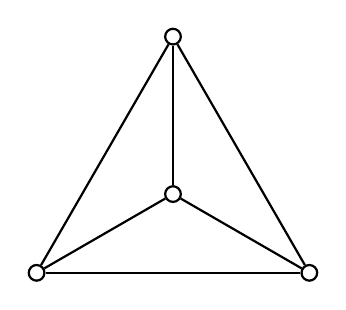
\begin{tikzpicture}
[nodedecorate/.style={shape=circle,inner sep=2pt,draw,thick},%
  linedecorate/.style={-,thick},%
  scale=2]
%% nodes or vertices
\foreach \nodename/\x/\y in {1/0.8660/-0.5, 2/0/1, 3/-0.8660/-0.5,
  4/0/0}
{
  \node (\nodename) at (\x,\y) [nodedecorate] {};
}
%% edges or lines
\path
\foreach \startnode/\endnode in {1/2, 1/3, 1/4, 2/3, 2/4, 3/4} {
  (\startnode) edge[linedecorate] node {} (\endnode)
};
\end{tikzpicture}
}
\quad
%%
%% wheel graph W_5
\subfigure[$W_5$]{
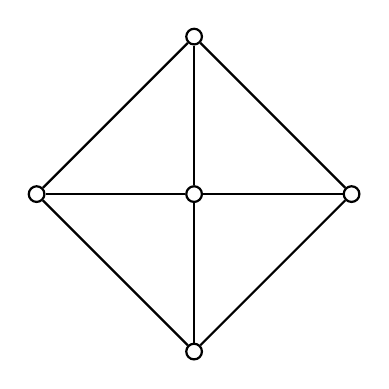
\begin{tikzpicture}
[nodedecorate/.style={shape=circle,inner sep=2pt,draw,thick},%
  linedecorate/.style={-,thick},%
  scale=2]
%% nodes or vertices
\foreach \nodename/\x/\y in {1/1/0, 2/0/1, 3/-1/0, 4/0/-1, 5/0/0} {
  \node (\nodename) at (\x,\y) [nodedecorate] {};
}
%% edges or lines
\path
\foreach \startnode/\endnode in {1/2, 1/4, 1/5, 2/3, 2/5, 3/4, 3/5,
  4/5}
{
  (\startnode) edge[linedecorate] node {} (\endnode)
};
\end{tikzpicture}
}
\quad
%%
%% wheel graph W_6
\subfigure[$W_6$]{
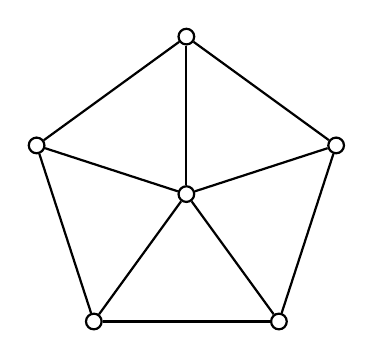
\begin{tikzpicture}
[nodedecorate/.style={shape=circle,inner sep=2pt,draw,thick},%
  linedecorate/.style={-,thick},%
  scale=2]
%% nodes or vertices
\foreach \nodename/\x/\y in {1/0.9510/0.3090, 2/0/1, 3/-0.9510/0.3090,
  4/-0.5877/-0.8090, 5/0.5877/-0.8090, 6/0/0}
{
  \node (\nodename) at (\x,\y) [nodedecorate] {};
}
%% edges or lines
\path
\foreach \startnode/\endnode in {1/2, 1/5, 1/6, 2/3, 2/6, 3/4, 3/6,
  4/5, 4/6, 5/6}
{
  (\startnode) edge[linedecorate] node {} (\endnode)
};
\end{tikzpicture}
}
%%
%% wheel graph W_7
\subfigure[$W_7$]{
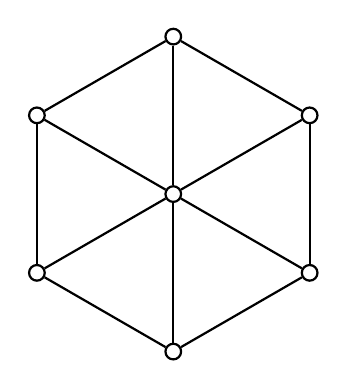
\begin{tikzpicture}
[nodedecorate/.style={shape=circle,inner sep=2pt,draw,thick},%
  linedecorate/.style={-,thick},%
  scale=2]
%% nodes or vertices
\foreach \nodename/\x/\y in {1/0.8660/0.5, 2/0/1, 3/-0.8660/0.5,
  4/-0.8660/-0.5, 5/0/-1, 6/0.8660/-0.5, 7/0/0}
{
  \node (\nodename) at (\x,\y) [nodedecorate] {};
}
%% edges or lines
\path
\foreach \startnode/\endnode in {1/2, 1/6, 1/7, 2/3, 2/7, 3/4, 3/7,
  4/5, 4/7, 5/6, 5/7, 6/7}
{
  (\startnode) edge[linedecorate] node {} (\endnode)
};
\end{tikzpicture}
}
\quad
%%
%% wheel graph W_8
\subfigure[$W_8$]{
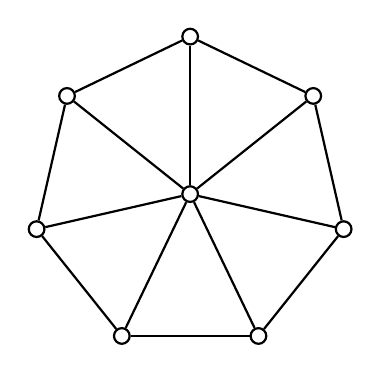
\begin{tikzpicture}
[nodedecorate/.style={shape=circle,inner sep=2pt,draw,thick},%
  linedecorate/.style={-,thick},%
  scale=2]
%% nodes or vertices
\foreach \nodename/\x/\y in {1/0.7818/0.6234, 2/0/1, 3/-0.7818/0.6234,
  4/-0.9749/-0.2225, 5/-0.4338/-0.9009, 6/0.4338/-0.9009,
  7/0.9749/-0.2225, 8/0/0}
{
  \node (\nodename) at (\x,\y) [nodedecorate] {};
}
%% edges or lines
\path
\foreach \startnode/\endnode in {1/2, 1/7, 1/8, 2/3, 2/8, 3/4, 3/8,
  4/5, 4/8, 5/6, 5/8, 6/7, 6/8, 7/8}
{
  (\startnode) edge[linedecorate] node {} (\endnode)
};
\end{tikzpicture}
}
\quad
%%
%% wheel graph W_9
\subfigure[$W_9$]{
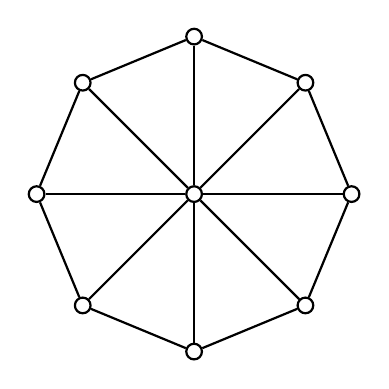
\begin{tikzpicture}
[nodedecorate/.style={shape=circle,inner sep=2pt,draw,thick},%
  linedecorate/.style={-,thick},%
  scale=2]
%% nodes or vertices
\foreach \nodename/\x/\y in {1/1/0, 2/0.7071/0.7071, 3/0/1,
  4/-0.7071/0.7071, 5/-1/0, 6/-0.7071/-0.7071, 7/0/-1,
  8/0.7071/-0.7071, 9/0/0}
{
  \node (\nodename) at (\x,\y) [nodedecorate] {};
}
%% edges or lines
\path
\foreach \startnode/\endnode in {1/2, 1/8, 1/9, 2/3, 2/9, 3/4, 3/9,
  4/5, 4/9, 5/6, 5/9, 6/7, 6/9, 7/8, 7/9, 8/9}
{
  (\startnode) edge[linedecorate] node {} (\endnode)
};
\end{tikzpicture}
}
\end{figure}

\end{document}
